%!TEX TS-program = xelatex
\documentclass[]{friggeri-cv}
\usepackage{graphicx}
\addbibresource{bibliography.bib}

\begin{document}
\header{Olivier }{Gayot}
       {4th-year student}


% In the aside, each new line forces a line break
\begin{aside}
    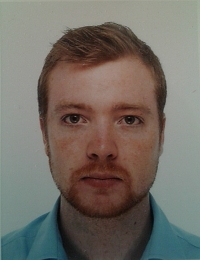
\includegraphics[width=100pt]{photo.png}
  \section{about}
    Woolf College
    CT2 7BQ
    United Kingdom
    --
    21 years old
    Driving License
    --
    ~
    phone: +33663613699
    \href{mailto:ogayot@free.fr}{ogayot@free.fr}
    \href{https://github.com/duskCoder}{github: duskCoder}
    \href{http://www.sigexec.com}{http://www.sigexec.com}
  \section{languages}
    french: mother tongue
    english: fluent
\end{aside}

\section{Experience}

\begin{entrylist}
  \entry
    {Apr. 2014 \\-> Sep. 2014}
    {BayLibre, Valbonne - Sophia Antipolis (France)}
    {Placement}
    {\emph{Portage of the latest versions of the Linux Kernel and Android to the BeagleBone Black. Contribution to a Power Cape project for the same board.}}
  \entry
    {Oct. 2013 \\-> Feb. 2014}
    {Fun RC Toys, Nancy Area (France)}
    {Partnership for a study project}
    {\emph{Development of a module of safety for drones (i.e. quadricopters) with three other students}}
  \entry
    {Oct. 2013 \\-> May 2014}
    {Intersec, Paris (France)}
    {Part time software developer}
    {\emph{Improvement of the software I developed during my placement (see below)}}
  \entry
    {Jul. 2012 \\-> Dec. 2012}
    {Intersec, Paris (France)}
    {Placement within the R\&D department}
    {\emph{Development of a software capable of simulating the motions of a large network of subscribers who move smartly inside a given zone}}
\end{entrylist}

\section{Interests}

Low level programming\\
Computer security (exploitation and prevention)\\
Embedded development\\
Open Source development\\
Discovery of new technologies

\section{Education}

\begin{entrylist}
  \entry
    {Sept. 2014\\-> Expected 2015}
    {Master degree of Science}
    {University of Kent, England}
    {Course of Computer Security}
  \entry
    {Juil. 2014\\-> Expected 2016}
    {Master degree of Information Technology}
    {EPITECH Paris, France}
    {}
  \entry
    {Oct. 2011\\-> Jul. 2014}
    {Bachelor degree of Information Technology}
    {EPITECH Nancy, France}
    {}
  \entry
    {2011}
    {French Baccalauréat S. with honours}
    {Lycée Raymond Poincaré, France}
    {Specialized in Sciences of the Engineer}
\end{entrylist}

\section{Technologies}
\begin{entrylist}
  \entry
    {C}
    {Proficient}
    {}
    {Heavy use of the C99 standard and the GNU extensions}
  \entry
    {C++}
    {Intermediate}
    {}
    {Fairly good Object-Oriented Thinking}
\end{entrylist}      % XXX
\begin{entrylist}    % move this block above another entry to wrap correctly
  \entry
    {Assembly}
    {Intermediate}
    {}
    {IA-32 and x86\_64 instruction sets\\
    writing and reverse engineering}
  \entry
    {Web}
    {Appropriate knowledge of common web-related technologies}
    {}
    {XHTML/CSS\\
        Server-side scripting: PHP\\
        Client-side scripting: JavaScript (+ jQuery)
    }
  \entry
    {Python 2\&3}
    {Beginner}
    {}
    {Currently writing a wrapper for the libelf in order to learn the language}
  \entry
    {Perl}
    {Beginner}
    {}
    {}
\end{entrylist}
\section{Software}
\begin{entrylist}
  \entry
    {}
    {Daily use of GNU/Linux, occasional use of Microsoft Windows}
    {}
    {Heavy usage of Vim\\
    (D)CVS: Git, Subversion\\
    GNU Autotools, make, GCC\\
    Debugging: gdb, valgrind, ollydbg}

\end{entrylist}

\section{Miscellaneous}
\begin{entrylist}
  \entry
    {}
    {}
    {}
    {Understanding of the ELF file format\\
    Active membre of the ASEN (\emph{Association de Sécurité d'EPITECH Nancy})\\
    Good knowledge of the benefits and pitfalls related to the use of unsafe languages (e.g. C)}
\end{entrylist}

\end{document}
